Figma es una herramienta de diseño gráfico en línea que se utiliza para crear
interfaces de usuario, diseños de sitios web, aplicaciones móviles y otros
proyectos digitales. Fue lanzado en 2016 y se ha vuelto muy popular en la
industria del diseño debido a su capacidad para trabajar en tiempo real y
permitir la colaboración en tiempo real entre los miembros del equipo.
\begin{figure}[htb!]
    \centering
    \caption{Logo de Figma}
    \label{fig:figma-logo}
    \centering
    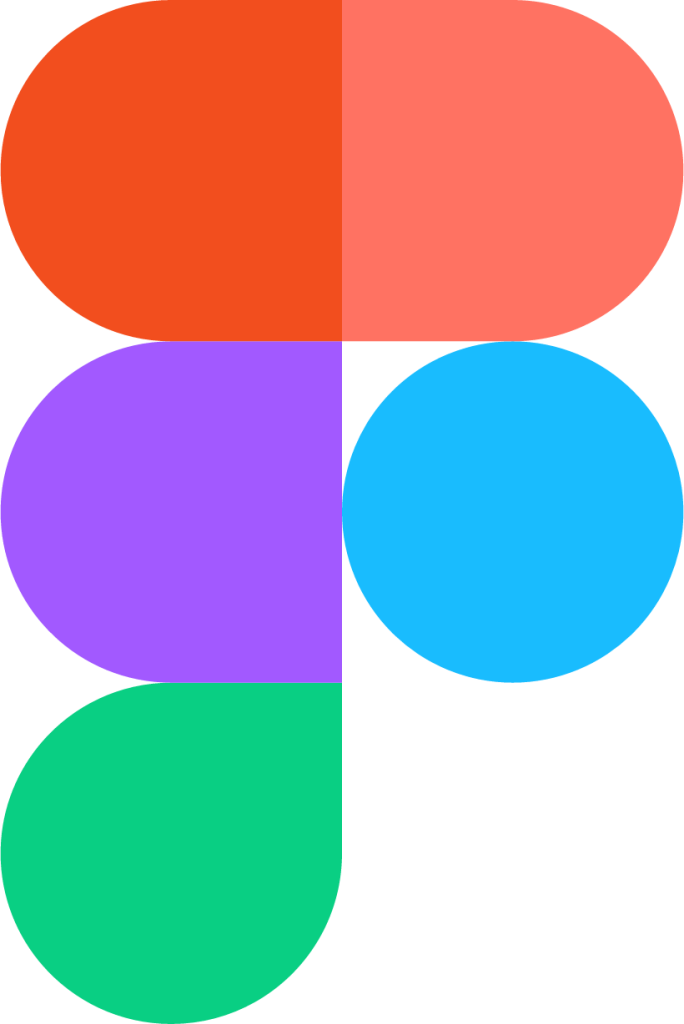
\includegraphics[scale=0.05]{./Ilustraciones/logos/figma.684x1024.png}\\
    \textbf{Fuente:} Iconduck [\url{https://iconduck.com/icons/39864/figma}]
\end{figure}
Figma nos permite crear diseños con herramientas como vectores,
formas, capas, texto y efectos, entre otras. También tiene características como
prototipado y animación, lo que lo hace ideal para diseñar interfaces interactivas.

Además, Figma es una herramienta basada en la nube, lo que significa que todos
los archivos se guardan en línea y se pueden acceder desde cualquier lugar con
conexión a Internet. Esto permite la colaboración en tiempo real entre los
miembros del equipo, ya que varios diseñadores pueden trabajar en un proyecto
simultáneamente y realizar cambios que se actualizan en tiempo real.